\chapter{Experiments}

\section{AE vs VAE}

Since our main goal is to create an end-to-end RL algorithm composed of an encoder followed by SAC we first need to decide wheter to use an autoencoder or a variational autoencoder. In other words, we want to explore if the stochasticity of a VAE can help in learning a good representation of the actual state. In order to do so, we follow a simple approach, train multiples both AEs and VAEs to see how much information they are able to recover from the latent vector with an MSE loss on average. As described above, we run a single pre-train on the dataset and then the chosen encoder remains unchanged for the entire duration of the RL agent training. There are varius choices that must be made before proceeding with the RL training. Firts we have to choose between AE and VAE, then the size of the latent vector $z$ and finally wheter to use data augmentation or not to improve the generalization of our model. In particular we consider an AE and a VAE network composed as respectively described in Listings \ref{lst:aenet} and \ref{lst:vaenet}. In Tables \ref{tab:aesim},\ref{tab:aereal}, \ref{tab:vaesim},\ref{tab:vaereal} are shown the result of trainings, each encoder has been trained three times to increase the reliability of the results and the average is reported in the tables. As we see in all cases the encoder performs better when augmentation is disabled, furthermore increasing z\_size to 64 dimensions results in a better reconstruction loss. Finally, the VAE performs slightly better then AE. In figure \ref{fig:realvaeexample} is shown what the reconstructed images looks like for the chosen VAE trained without augmentation and a latent vector size of 64 dimension. All the other encoder reconstructions are shown in APPENDIX TODO.

\begin{figure}[h]
  \begin{minipage}{.50\textwidth}
    \centering
    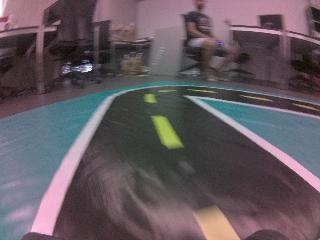
\includegraphics[height=0.50\textwidth]{experiments/11296.jpg}
  \end{minipage}%
  \begin{minipage}{.50\textwidth}
      \centering
      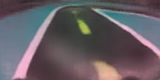
\includegraphics[width=0.60\textwidth]{experiments/11296.png}
  \end{minipage}
  \captionof{figure}{Real world image processed after cropping with a VAE, z\_size=64 and no augmentation. Reconstruction\_loss=112}
  \label{fig:realvaeexample}
\end{figure}
\begin{figure}
  \begin{minipage}{.50\textwidth}
    \centering
    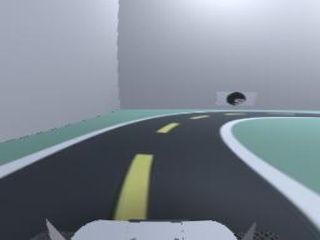
\includegraphics[height=0.50\textwidth]{experiments/1160.jpg}
  \end{minipage}%
  \begin{minipage}{.50\textwidth}
      \centering
      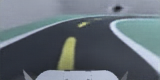
\includegraphics[width=0.60\textwidth]{experiments/1160.png}
  \end{minipage}
  \captionof{figure}{Simulator image processed after cropping with a VAE, z\_size=64 and no augmentation. Reconstruction\_loss=17}
  \label{fig:simvaeexample}
\end{figure}

\begin{table}
  \centering
  \begin{tabular}{|c|c||c|c|c|c|}
  \hline
  Z\_SIZE & AUGMENTATION & MEAN & STD & MAX & MIN \\ \hline
  \multirow{2}{*}{32} & False & 121.54 & 102.42 & 795.44 & 45.61 \\
  & True & 164.57 & 95.51 & 783.03 & 65.13  \\ \hline
  \multirow{2}{*}{64} & False & 103.54 & 79.14 & 588.14 & 40.84 \\
  & True & 137.24 & 74,02 & 611,81 & 63,05  \\ \hline
  \end{tabular}
  \caption{AE trained in simulation - reconstruction loss}
  \label{tab:aesim}

  \begin{tabular}{|c|c||c|c|c|c|}
  \hline
  Z\_SIZE & AUGMENTATION & MEAN & STD & MAX & MIN \\ \hline
  \multirow{2}{*}{32} & False & 377.07 & 87.53 & 756.7 & 239.46 \\
  & True & 493.84 & 99.40 & 807.67 & 289.99  \\ \hline
  \multirow{2}{*}{64} & False & 311.1 & 78.5 & 695.65 & 177.77 \\
  & True & 411.37 & 77.30 & 647.68 & 241.87 \\ \hline
  \end{tabular}
  \caption{AE trained in real world - reconstruction loss}
  \label{tab:aereal}

  \begin{tabular}{|c|c||c|c|c|c|}
  \hline
  Z\_SIZE & AUGMENTATION & MEAN & STD & MAX & MIN \\ \hline
  \multirow{2}{*}{32} & False & 59.1 & 60.41 & 620.93 & 18.88 \\
  & True & 116.31 & 71.11 & 771.88 & 51.10  \\ \hline
  \multirow{2}{*}{64} & False & 45.15 & 43.49 & 480.22 & 14.34 \\
  & True & 112.17 & 59.79 & 573.19 & 54.28  \\ \hline
  \end{tabular}
  \caption{VAE trained in simulation - reconstruction loss}
  \label{tab:vaesim}

  \begin{tabular}{|c|c||c|c|c|c|}
  \hline
  Z\_SIZE & AUGMENTATION & MEAN & STD & MAX & MIN \\ \hline
  \multirow{2}{*}{32} & False & 227.4 & 44.74 & 418.7 & 140.12 \\
  & True & 263.87 & 52.29 & 478.26 & 172.70 \\ \hline
  \multirow{2}{*}{64} & False & 184.56 & 36.86 & 347.59 & 96.7 \\
  & True & 230.66 & 42.24 & 402.67 & 156.61  \\ \hline
  \end{tabular}
  \caption{VAE trained in real world - reconstruction loss}
  \label{tab:vaereal}
\end{table}


\begin{center}
    \begin{minipage}{0.9\linewidth}
      \lstinputlisting[caption=AE network, label=lst:aenet]{ae.txt}
      \end{minipage}
    \begin{minipage}{0.9\linewidth}
      \lstinputlisting[caption=VAE network, label=lst:vaenet]{vae.txt}
      \end{minipage}
\end{center}

\section{RL algorithm}

\subsection{Reward function}
Designing a reward function that can work on both simulated and real environments is not trivial. In simulation, the environment can provide a better supervision than a human can do. In our real setup we have only the camera frames as states and so no other sensor is available, even though they can be used. In simulation, instead, the environment can tell us how far the donkeycar is from the center line of the track, with this value, we can decrease the reward function by a value proportional to the distance of the car from the center of the roadway as done in Equation \ref{eq:stdreward}. So the reward function is:

\begin{equation}
  \label{eq:stdreward}
  r_t = 1 + throttle\_reward + cte\_penalty
\end{equation}
where 1 is given for each step taken by the agent in order to incentivize the completion of the largest possible number of steps. The throttle reward incentives the car to go as fast as possible, however in our setup, the throttle is kept constant for the purposes of this thesis. Finally the Cross Track Error (CTE) penalty, is a negative value to incentive the car to stay as close as possibile to the center of the roadway. In case the car exceeds a predefined maximum CTE, the penalty becomes very high and the episode ends. 
This first reward function is used to test our algorithm and after proving it can work, we need to adapt it such that it can work also in real world. To tackle the issue we simply replace the CTE penalty with a negative value to be activated only when an episode ends due to human intervention. The final reward function that has proven to work in both environment and we use in our trainings is:

\begin{equation}
  \label{eq:realreward}
  r_t = 1 + throttle\_reward + off\_track
\end{equation}
Another reward function was initally tested trying to improve the total time an agent takes to complete a lap:
\begin{equation}
  \label{eq:testreward}
  r_t = - 0.1 + throttle\_reward + cte\_penalty
\end{equation}
The idea behind this function is that any step gives a negative reward and thus the agent must finish a lap in the smallest number of step to maximize the total episode reward. Minimizing the number steps means also finding the shortest way and consequently reducing the total time spent for a lap. Unfortunately, this approach did not let the agent learn to drive decently, at least in reasonable time.

\subsection{Training the simulated RL agent}
As a baseline for RL algorithm we used the source code provided by \citet{DBLP:journals/corr/abs-2008-00715}. His algorithm allows both simulated and real training, however training on simulation with communication being over-the-internet is more computationally expensive and more prone to errors. Thus, for the simulation, we refactor the algorithm such that the communication happens locally. Beside that, his algorithm uses an AE which need to be changed with the VAE chosen above. Given that the simulator provides several training modality we need to test them to find out which one is the best, to eventually save time in real world. We can chose where car starts and also where the laps ends. 

% After varius tests we found convinent in terms of learning speed to cyclically use all the checkpoints with the modality described in Section \ref{sec:track}. The learning procedure in simulation is simple, the agent starts on a given checkpoint and keep moving until the simulator does not notify that the DonkeyCar crashed or exceed more than a certain value the roadway.

\subsection{Training the real RL agent}
In real world instead we keep the source code provided by \citet{DBLP:journals/corr/abs-2008-00715} untouched. And the main goal is to replicate the results but with a more performing encoders as resulted in our tests. 

\section{Sim to Real}